\chapter{\label{ch:experiments}Experiments}
In this chapter, we will describe the experiments we made and present the
results we obtained. In Section~\ref{sec:clone-detection-experiments}, we will
present our experiments about code clone detection, while in
Section~\ref{sec:token-generation-experiments} we will describe our experiments
to generate token embedding. In both sections we will show what kind of data we
used to train our model and how our model perform with different
hyper-parameters.

To run our experiments, we used the two machines shown in
table~\ref{tab:machine-specs}. In table~\ref{tab:softwares}, we show the
softwares we used to implement and run our machine-learning related experiments
and the version we used.

\begin{table}
  \caption{\label{tab:machine-specs}Machines used for experiments}
  \begin{center}
    \begin{tabular}{r c c}
      \toprule
       & Machine 1 & Machine 2\\
      \toprule
      \textbf{CPU} & Intel i7-6850K & Intel Xeon E5-2637 v3\\
      \textbf{CPU frequency} & 3.60GHz & 3.50GHz\\
      \textbf{Cores count} & 6 & 8\\
      \textbf{Threads count} & 12 & 16\\
      \textbf{Memory} & 64GB & 512GB\\
      \textbf{GPU} & Nvidia Quadro P6000 & Nvidia Tesla K40\\
      \textbf{GPU memory} & 24GB & 16GB\\
      \bottomrule
    \end{tabular}
  \end{center}
\end{table}
%
\begin{table}
  \caption{\label{tab:softwares}Softwares used for experiments}
  \begin{center}
    \begin{tabular}{r c}
      \toprule
       Software & Version\\
      \toprule
      Linux & 4.14 / 4.4\\
      CUDA & 8.0\\
      cuDNN & 6.0\\
      Python & 3.6.2\\
      Tensorflow & 1.3.1\\
      Keras & 2.1.2\\
      \bottomrule
    \end{tabular}
  \end{center}
\end{table}
\section{\label{sec:clone-detection-experiments}Code clone detection}
To evaluate our clone detection model, we implemented the model we described
in~\ref{sec:clone-detection}, we collected data of programs implementing the
same functionality to feed to the model, and we trained and evaluated our model
with different hyper-parameters. In this section, we will give some details
about the data we collected for our experiments and present the different
results we obtained when evaluating our model.
\subsection{\label{ssec:clone-detection-dataset}Code clone detection dataset}
As we are using a supervised learning approach to code clone detection, to train
our model we needed data which fulfills the following properties.

\begin{enumerate}
\item Multiple code fragments should implement the same functionality
\item Information on whether two code fragments implement the same functionality
  must be included
\item Dataset should contain code fragments written in at least 2 programming
  languages
\end{enumerate}

To the best of our knowledge, no dataset currently available fulfills all the
necessary properties to our experiments, therefore we created our own dataset.

For this dataset, we found that competitive programming websites are an
excellent match. The solution to a single problem is implemented by a
large number of persons in many different languages. All the solutions to a
single problem must implement exactly the same functionality, therefore,
we are assured that all source codes implementing a solution to the same problem
are at least type IV code clones. The easier the problem is, the higher the
probability of code fragments implementing the solution to the same problem have
to be very similar to each other, and to therefore be closer to type III clones.
Furthermore, multiple solutions to a problem are always implemented by different
users, which makes our dataset closer to the motivating example we presented in
Section~\ref{sec:motivating-exmaple}.

To create the dataset, we scraped code from a famous Japanese competitive
programming website. As our implementation currently only supports Java and
Python, we fetched data for these two programming languages. We restricted the
data to only programs that were accepted by the website judging system --- meaning
that the programs actually implemented the solution to the given problem --- in
order to have the type IV code clone guarantee. In
table~\ref{tab:clone-dataset-overview}, we give some statistics about the
dataset we created and in table~\ref{tab:clone-dataset-languages} we show how
the given statistics are distributed between Python and Java. We show the
distribution of the number of files per problem --- which is representative of
the number of clones in the dataset --- in
figure~\ref{fig:files-per-problem-distribution}.

\begin{table}
  \caption{\label{tab:clone-dataset-overview} Clone detection dataset overview}
  \begin{center}
    \begin{tabular}{c c}
      \toprule
      Measure & Value\\
      \toprule
      Problems count & 576\\
      Avg. files / problem & 77\\
      Files count & 44620\\
      Lines count & 1270599\\
      Tokens count & 8554476\\
      \bottomrule
    \end{tabular}
  \end{center}
\end{table}

\begin{table}
  \caption{\label{tab:clone-dataset-languages} Clone detection dataset language overview}
  \begin{center}
    \begin{tabular}{c c c}
      \toprule
      & Python & Java\\
      \toprule
      Avg. files / problem & 41 & 36\\
      Files count & 23792 & 20828\\
      Lines count & 312353 & 958246\\
      Tokens count & 1810085 & 6744391\\
      \bottomrule
    \end{tabular}
  \end{center}
\end{table}

\begin{figure}
  \begin{center}
    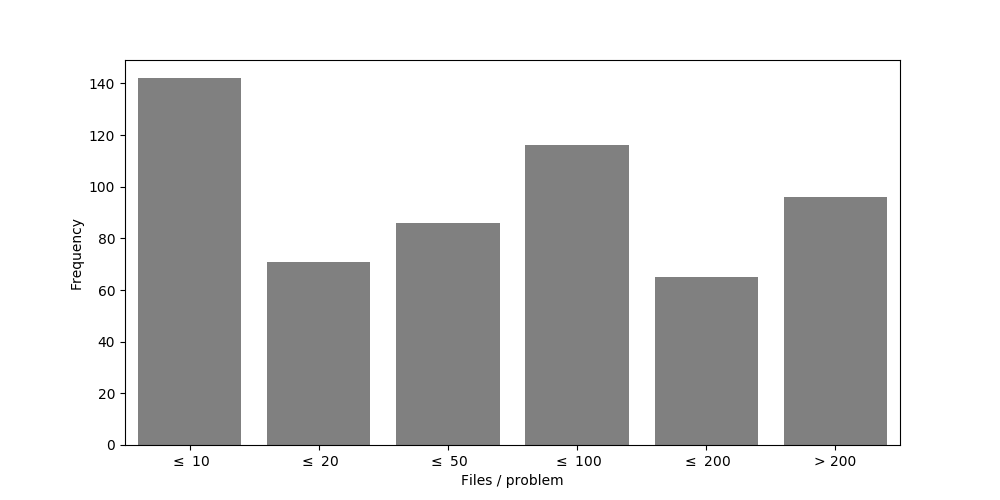
\includegraphics[width=16cm]{./images/code-clone-dataset-problems-distribution.png}
    \caption{\label{fig:files-per-problem-distribution} Distribution of the
      number of files per problem}
  \end{center}
\end{figure}

In order to be able to feed the code to our model, we transform the code we
fetched using \lstinline{bigcode-astgen} we presented in
Section~\ref{sec:ast-generation} using the commands shown in
listing~\ref{lis:atcoder-astgen}.

\begin{lstlisting}[numbers=none,language={},
  caption=AST generation using \lstinline{bigcode-astgen}, label=lis:atcoder-astgen]
bigcode-astgen-java --batch -f 'src/**/*.java' -o java-asts
bigcode-astgen-py --batch -f 'src/**/*.py' -o python-asts
cat java-asts.json python-asts.json > asts.json
cat java-asts.txt python-asts.txt > asts.txt
\end{lstlisting}
With the first two commands, we generate the ASTs for Python and Java source
files, and with the next we commands we merge the ASTs and the file which maps
the index of the AST in the JSON file to the name of the file in the original
dataset.
\subsection{\label{ssec:clone-detection-hyper-params}Code clone detection model hyper-parameters}
Our model contains many hyper-parameters that can vastly influence its
performances while detecting clones. In listing~\ref{lis:model-config}, we show a
sample configuration file that we actually use to train our model. The file is
written using in YAML and is loaded by our system when training and evaluating
the model. Although the file we show here is not complete, it contains the main
settings that one might want to change when training a model.

\begin{figure}
  \lstinputlisting[language={}, basicstyle=\ttfamily\footnotesize, caption=Model
  configuration file,label=lis:model-config]{./snippets/config.yml}
\end{figure}

We describe the meaning of each parameter in our configuration file in
table~\ref{tab:hyper-parameters}.

\begin{table}[p]
  \caption{\label{tab:hyper-parameters}Clone detection model hyper-parameters}
  \begin{center}
    \begin{tabularx}{\linewidth}{c c X l}
      \toprule
      Parameter & Notation & Description & Sample value\\
      \toprule
      \lstinline{transformer_class_name} & $f_t$ & The algorithm to used to encode
      the AST into a vector as described in~\ref{sssec:ast-transformer} & \lstinline{DFSTransformer}\\
      \lstinline{vocabulary} & & The path to the extracted vocabulary & \lstinline{vocab.tsv}\\
      \lstinline{vocabulary_size} & $|V|$ & The size of the vocabulary & $500$\\
      \lstinline{embeddings} & & The path to the trained token embedding. If
      this parameter is not provided, embedding are randomly initialized & \lstinline{embeddings.pickle}\\
      \lstinline{embeddings_dimension} & $d_w$ & Dimension of the embedding for
      target language & $100$\\
      \lstinline{output_dimensions} & $d_e$ & Dimension of the
      LSTM encoder. If the size is greater than $1$, the LSTM will be stacked
      and the output dimension will be the value of the last element of the list
      & \lstinline{[100, 50]}\\
      \lstinline{bidirectional_encoding} & $f_{e_b}$ & Whether or not to use a
      bidirectional LSTM & \lstinline{true}\\
      \lstinline{name} & & The name of the programming language & java\\
      \lstinline{input_length} & $|X|$ & The max. number of tokens per code
      fragment. This restriction can be avoided at the cost of a performance
      penalty & $1000$\\
      \lstinline{merge_mode} & $f_m$ & Algorithm to use to merge the two code
      fragments as described in~\ref{sssec:merge-layer} & bidistance
    \end{tabularx}
  \end{center}
\end{table}
\begin{table}[p]
  \begin{center}
    \begin{tabularx}{\textwidth}{c c X l}
      \lstinline{merge_output_dim} & $d_o$ & Output dimension to use for the
      merge layer. Currently only effective when using
      equation~\ref{eq:bidistance-merge-layer} as the merge layer & \lstinline{50}\\
      \lstinline{dense_layers} & $d(f_p)$ & The number of hidden layers to use for the
      final MLP and their number of units & \lstinline{[50, 50]}\\
      \lstinline{optimizer} & & The optimizer to use to train the model & rmsprop\\
      \lstinline{submissions_path} & & The path of the submissions metadata & \lstinline{submissions.json}\\
      \lstinline{asts_path} & & The path of the training data ASTs generated
      as described above & \lstinline{asts.json}\\
      \lstinline{split_ratio} & & The amount of data to use for training,
      hyper-parameter tuning, and testing the model & \lstinline{[0.8, 0.1, 0.1]}\\
      \lstinline{shuffle} & & Whether or not to shuffle the data when training
      the model & \lstinline{true}\\
      \lstinline{negative_samples} & $|S_n|$ & The number of non-clone noise data ---
      negative sample --- to generate per code clone & $4$\\
      \lstinline{negative_sample_distance} & $\Delta S_n$ & The maximum distance ratio
      between the size of the input and the size of the negative sample, to avoid
      the model to try to detect clones by number of tokens & $0.2$\\
      \lstinline{class_weights} & $L_w$ & The weight to assign to positive and
      negative samples. The higher the weight, the more an error will be
      penalized & \lstinline{\{0: 2.0, 1: 1.0\}}\\
      \lstinline{batch_size} &  & The size of a batch when training the model & $256$\\
      \lstinline{epochs} & & The number of epochs to train the model & $10$\\
      \bottomrule
    \end{tabularx}
  \end{center}
\end{table}
%
Although there is a very large number of hyper-parameters, not all affect our
model in the same way. For example, while the vocabulary we use, or the way we
transform the AST into a vector affects greatly the performance of the model,
other parameters such as the optimizer we use or the batch size do not are not
as important. We will explain more in detail how each section in our
configuration is used, and explain some of the decisions to be made when setting
these parameters.

The parameters under each object of the \lstinline{languages} section contains
the necessary information to encode an AST into a vector for the given
programming language. The vocabulary and embedding we pass will determine how
each token is encoded into its vector representation. We will discuss further
how these embedding are trained in
Section~\ref{sec:token-generation-experiments}, but the most important decision
being made for the embedding is if we want to use the values of the tokens or
simply their types, resulting in a small vocabulary in the order of $100$ tokens
in the first case, or a much larger vocabulary of thousands of tokens in the
second. The input length is the maximum number of tokens for a single code
fragment. We use this limit mainly for performance purpose, as we pad all the
inputs to this size to be able to train our model using batches. Given our
current implementation, removing this limits forces us to train the model a
sample at a time, largely hurting performance. This shortcoming can be mitigated
with techniques such as bucketing~\cite{DBLP:journals/corr/abs-1708-05604}, but
we leave this for future work. The \lstinline{output_dimensions} and
\lstinline{bidirectional_encoding} parameters control what kind of LSTM network
will be used to encode the vectorized AST into a single vector.

Other parameters under \lstinline{model} contain hyper-parameters on how the
input vectors should be merged, as well as what kind of network to use to
actually make the prediction. It also contains information about the optimizer
to use, and may have hyper-parameters for the optimizer such as its learning
rate.

The part under \lstinline{generator} contains all the information necessary to
generate data to train the model. \lstinline{submissions_path} and
\lstinline{asts_path} are the paths to the submissions metadata and their
encoded AST and all the data to train and evaluate the model will be loaded from
their. The negative samples related settings as well as the class weights mostly
affect the precision-recall trade-off, which we will discuss more in detail
in~\ref{ssec:clone-detection-experiment}.
\subsection{\label{ssec:clone-detection-experiment}Clone detection experiment}
In this section, we will describe the experiments we run to evaluate our clone
detection model.
We will here describe the experiment we run, show the results and give an
interpretation of the results we obtained.

First, we prepared the dataset to train our model by splitting the data we
described in~\ref{ssec:clone-detection-dataset} into training set containing
80\% of the data, the cross-validation set used to tune our hyper parameters
containing 10\% of the data, and finally the test set used to give a final
evaluation of our model. For both training, cross-validation and test, we treat
files implementing a solution to the same problem as clones, and randomly choose
$n$ samples from files implementing a solution to a different problem to use as
negative inputs to our model. We make the number of samples vary during training
but fix this number to $4$ samples for cross-validation, in order to be able to
compare the performance of the different models on the same input data.

We trained models to detect clone between Java and Python source code, as well
as models to perform clone detection between source fragments written in Java.
The main motivation for trying to run clone detection is Java is to be able to
compare our results with other clone detection tools. In
tables~\ref{tab:java-python-model-params} and~\ref{tab:java-java-model-params},
we show the hyper parameters we used for training models for respectively
Java/Python code clone detection and Java/Java code clone detection. Given the
large number of parameters which we tried when training the models, we only show
a subset including models which yielded the best results, as wee as models which
we would like to discuss further in the results interpretation. Our models are
sorted using the F1-score. In tables~\ref{tab:java-python-model-results}
and~\ref{tab:java-java-model-results}, we show different metrics for each model
when tested on the cross-validation set.

\begin{table}
  \caption{\label{tab:java-python-model-params}Java/Python clone detection
    models parameters}
  \begin{center}
    \begin{tabularx}{\linewidth}{c Y c Y c Y c c Y Y c c}
      \toprule
      $n$ & $|V|$ & $d_w$ & $d_e$ & $f_{e_b}$ & $d(f_p)$ & $f_t$ & $|S_n|$ & $L_w$ & $f_m$ & $\Delta S_n$\\
      \toprule
      $1$ & $10000$ & $100$ & $\{100,50\}$ & $t$ & $\{64\}$ & $f_{t_1}$ & $4$ & $\{1.0,1.0\}$ & $f_{m_2}$ & $0.2$\\
      $2$ & $10000$ & $100$ & $\{50,50\}$ & $t$ & $\{64\}$ & $f_{t_1}$ & $4$ & $\{1.0,1.0\}$ & $f_{m_2}$ & $0.2$\\
      $3$ & $10000$ & $100$ & $\{50\}$ & $t$ & $\{64\}$ & $f_{t_1}$ & $4$ & $\{1.0,1.0\}$ & $f_{m_2}$ & $0.2$\\
      $4$ & $-$ & $50$ & $\{50\}$ & $t$ & $\{64,64\}$ & $f_{t_1}$ & $2$ & $\{1.0,1.0\}$ & $f_{m_1}$ & $-$\\
      $5$ & $-$ & $50$ & $\{50\}$ & $t$ & $\{64,64\}$ & $f_{t_1}$ & $1$ & $\{1.0,1.0\}$ & $f_{m_1}$ & $-$\\
      $6$ & $-$ & $50$ & $\{100,50\}$ & $t$ & $\{64\}$ & $f_{t_1}$ & $4$ & $\{1.0,1.0\}$ & $f_{m_2}$ & $0.2$\\
      \bottomrule
    \end{tabularx}
  \end{center}
\end{table}
%
\begin{table}
  \caption{\label{tab:java-python-model-results}Java/Python clone detection
    models results}
  \begin{center}
    \begin{tabularx}{\linewidth}{c Y Y Y Y}
      \toprule
      $n$ & F1-score & Precision & Recall & Accuracy\\
      \toprule
      $1$ & $0.66$ & $0.55$ & $0.83$ & $0.83$\\
      $2$ & $0.63$ & $0.51$ & $0.80$ & $0.80$\\
      $3$ & $0.56$ & $0.42$ & $0.82$ & $0.73$\\
      $4$ & $0.55$ & $0.40$ & $0.84$ & $0.71$\\
      $5$ & $0.52$ & $0.38$ & $0.84$ & $0.68$\\
      $6$ & $0.49$ & $0.35$ & $0.80$ & $0.66$\\
      \bottomrule
    \end{tabularx}
  \end{center}
\end{table}
%
\begin{table}
  \caption{\label{tab:java-java-model-params}Java/Java clone detection
    models parameters}
  \begin{center}
    \begin{tabularx}{\linewidth}{c Y c Y c Y c c Y Y c c}
      \toprule
      $n$ & $|V|$ & $d_w$ & $d_e$ & $f_{e_b}$ & $d(f_p)$ & $f_t$ & $|S_n|$ & $L_w$ & $f_m$ & $\Delta S_n$\\
      \toprule
      $1$ & $10000$ & $100$ & $\{100,50\}$ & $t$ & $\{64\}$ & $f_{t_1}$ & $4$ & $\{1.0,1.0\}$ & $f_{m_2}$ & $0.2$\\
      $2$ & $10000$ & $100$ & $\{50\}$ & $t$ & $\{64\}$ & $f_{t_1}$ & $4$ & $\{1.0,1.0\}$ & $f_{m_2}$ & $0.2$\\
      $3$ & $10000$ & $30$ & $\{50\}$ & $t$ & $\{64\}$ & $f_{t_1}$ & $4$ & $\{1.5,1.0\}$ & $f_{m_2}$ & $0.2$\\
      $4$ & $10000$ & $30$ & $\{50\}$ & $t$ & $\{64\}$ & $f_{t_1}$ & $4$ & $\{2.0,1.0\}$ & $f_{m_2}$ & $0.2$\\
      $5$ & $10000$ & $30$ & $\{50\}$ & $t$ & $\{64\}$ & $f_{t_1}$ & $4$ & $\{1.0,1.0\}$ & $f_{m_2}$ & $0.2$\\
      $6$ & $-$ & $50$ & $\{30\}$ & $t$ & $\{64\}$ & $f_{t_1}$ & $1$ & $\{1.0,1.0\}$ & $f_{m_2}$ & $0.2$\\
      \bottomrule
    \end{tabularx}
  \end{center}
\end{table}
%
\begin{table}
  \caption{\label{tab:java-java-model-results}Java/Java clone detection
    models results}
  \begin{center}
    \begin{tabularx}{\linewidth}{c Y Y Y Y}
      \toprule
      $n$ & F1-score & Precision & Recall & Accuracy\\
      \toprule
      $1$ & $0.77$ & $0.67$ & $0.92$ & $0.89$\\
      $2$ & $0.76$ & $0.67$ & $0.88$ & $0.89$\\
      $3$ & $0.72$ & $0.64$ & $0.82$ & $0.87$\\
      $4$ & $0.69$ & $0.56$ & $0.89$ & $0.84$\\
      $5$ & $0.66$ & $0.53$ & $0.88$ & $0.82$\\
      $6$ & $0.55$ & $0.39$ & $0.94$ & $0.69$\\
      \bottomrule
    \end{tabularx}
  \end{center}
\end{table}

In tables~\ref{tab:java-python-model-params}
and~\ref{tab:java-java-model-params}, having $-$ in the $|V|$ column means that
we did not use the values of the tokens, and we did not have to limit the size
of the vocabulary as it was already small enough. Concretely, the vocabulary
size was of $130$ for Python and of $75$ for Java.

In general, our model gives us a high recall but does not manage to get a high
precision, especially for the cross-language classification task. These results
can be mitigated by trading recall for precision, but given the goal of our
model to find possible duplicates across systems, we prefer to keep a high
recall and leave the false-positive judgment to the developer. Furthermore, some
source code which are actually not clones do look very similar, and can
therefore be difficult to classify. For example, a code implementing Fibonacci
and a code implementing factorial both contain a main for loop, which does some
arithmetic operation and finally return an integer. Although the codes are not
doing exactly the same thing, and are therefore not clones, they contain enough
similarities to possibly be factorized, so the evaluation here could be a little
pessimistic.

From the hyper-parameters point of view, the main conclusion to draw from the
results we obtained is that when we do not include the values of the tokens and
try to train our model with only the types, the resulting model does not contain
enough information to be able to correctly detect clones and we have a large
drop in the precision score.
Another conclusion that we can draw from our results is that increasing the size
of the LSTM encoder improves the performance of the model. Especially for
cross-language detection, where the detection task is more difficult, we get a
considerable improvement by using a stacked LSTM instead of a simple one.
On the other hand, using algorithm $f_{t_2}$, which performs two depth-first
search, for transforming our ASTs into vectors yielded performance much worse
that the simple $f_{t_1}$ which only perform a single one. We suspect that
adding the result of the second depth-first search to the vector encoding added
more noise to the encoded data that it added information, but a more formal
conclusion about this result needs further investigation. We did not observe any
significant improvement by changing the size of the output MLP classifier, and
therefore concluded that the model performance was rather dependent on how we
encode the AST into a vector rather the classification of the encoded vectors. 
\section{\label{sec:token-generation-experiments}Token embedding generation}
To generate token vector embedding and evaluate our results, we implemented the
model and tools we described in Section~\ref{sec:token-representation}. All the
tools implemented to generated token embedding are publicly available on
GitHub\footnote{\url{https://github.com/tuvistavie/bigcode-tools}}, and made
available through pip when
possible\footnote{\url{https://pypi.python.org/pypi/bigcode-fetcher}}
\footnote{\url{https://pypi.python.org/pypi/bigcode-embeddings}}.
%
\subsection{Embedding generation dataset}
As described in Section~\ref{sec:token-representation}, data generation for
token embedding is unsupervised, as opposed to the approach we take for clone
detection. Getting data to train our model is therefore much easier. To train
embedding for a particular programming language, the only thing we need is a
large quantity of code written in this given language. This code should also be
as much as possible diverse so we can capture the tokens of most major libraries
and get a descent vector representation for their tokens.

To generate datasets to train token embedding for Python and Java, we fetched
code from GitHub using our \lstinline{bigcode-embeddings} tool, and then
generated the ASTs for all the files using \lstinline{bigcode-astgen}.
For Java, we chose to use all the projects written in Java and belonging to The
Apache Software Foundation\footnote{\url{http://www.apache.org/}}. For Python,
as we could not find any organization with a sufficient amount of source code,
we projects which fulfilled the following conditions.

\begin{itemize}
\item Size between 100KB and 100MB
\item Non-viral license (e.g. MIT, BSD)
\item Not forks
\end{itemize}

We ordered the results by number of stars as a proxy of the popularity of the
project and kept all the files which contained more than 10 tokens and less than
10000 tokens. Although our AST generation tool supports both Python 2 and Python
3, the produced AST may vary slightly and we therefore decided to use only
Python 3 for this experiment.

We show some metrics for our Java dataset in
table~\ref{tab:java-embedding-dataset} and for our Python dataset in
table~\ref{tab:python-embedding-dataset}.

\begin{table}
  \caption{\label{tab:java-embedding-dataset}Embedding generation Java dataset
    metrics}
  \begin{center}
    \begin{tabular}{r r}
      \toprule
      Metric & Value\\
      \toprule
      Projects count & 1,027\\
      Files count & 476,685\\
      Lines count & 80,367,840\\
      Tokens count & 301,930,231\\
      \bottomrule
    \end{tabular}
  \end{center}
\end{table}

\begin{table}
  \caption{\label{tab:python-embedding-dataset}Embedding generation Python
    dataset metrics}
  \begin{center}
    \begin{tabular}{r r}
      \toprule
      Metric & Value\\
      \toprule
      Projects count & 879\\
      Files count & 131,506\\
      Lines count & 55,796,594\\
      Tokens count & 89,757,436\\
      \bottomrule
    \end{tabular}
  \end{center}
\end{table}

\subsection{Vocabulary generation results}
As discussed in Section~\ref{sec:token-representation}, the first step when
creating token embedding is to generate a vocabulary for the given programming
language. We will here present the results for the different vocabularies we
generated. For both Java and Python, we generated 3 different kinds of
vocabularies:

\begin{enumerate}
\item Vocabulary without token values
\item Vocabulary of $500$ tokens with values
\item Vocabulary of $10000$ tokens with values
\end{enumerate}

The vocabulary without token values only contains only the type of each token,
for example, \lstinline{ImportStmt} in Java, or \lstinline{FunctionDef} in
Python. In figures~\ref{fig:no-values-vocabulary-distribution}
to~\ref{fig:with-values-vocabulary-distribution}, we show the relation between
the rank of a token in the vocabulary, and its number of appearances. We use a
log scale for both axes. An interesting property we find is that, when using
values of the tokens, this relation and by extension the distribution of the
frequency tokens in a programming language follows the Zipf's
law~\cite{piantadosi2013zipf}, in the same way as natural languages do.
When we exclude the tokens, and therefore only use the type of each token to
generate the vocabulary, the law seems to hold only until the few last tokens of
each language, which indicates that there is a small number of types in each
language that are almost never used. Regardless of the fact that we use or not
values of each token, the distribution is almost the same for both Python and
Java, and the fact that the curve for Java is above the one for Python comes
from the fact that we extracted more tokens for Java and we did not normalize
the results, as it was not needed for the rest of the embedding generation.

Given the distribution of the token frequency in both programming languages
follow closely the frequency found in natural languages, we can expect that a
model such as skipgram which works well with natural languages to also work
here.

\begin{figure}
  \centering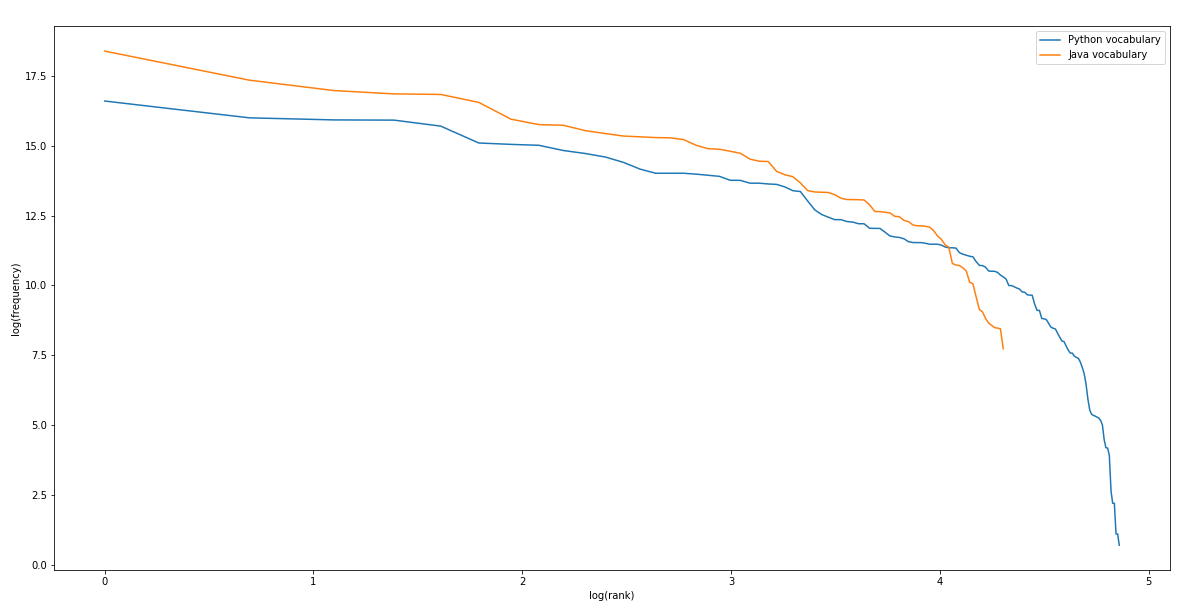
\includegraphics[width=14cm]{images/distribution-without-values.png}
  \caption{\label{fig:no-values-vocabulary-distribution}Tokens without value
    relation between token frequency and rank}
\end{figure}

\begin{figure}
  \centering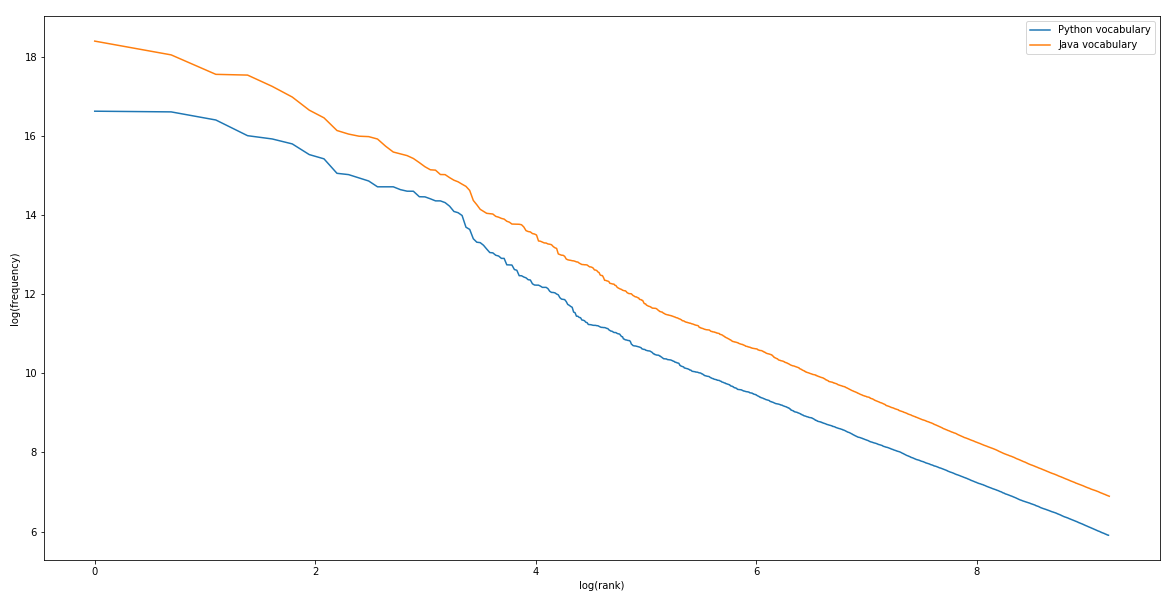
\includegraphics[width=14cm]{images/distribution-with-values.png}
  \caption{\label{fig:with-values-vocabulary-distribution}Tokens with value
    relation between token frequency and rank}
\end{figure}

\subsection{Embedding generation experiments}
Once we created our vocabulary, we want to assign a vector in $\mathbb{R}^{d_w}$
to each token in our vocabulary. Given the purpose of generating these embedding
is to encode a program so that we can detect clone, the main requirement of our
embedding is that tokens which are semantically similar, such that for example
\lstinline{while} and \lstinline{for} have a small distance, while unrelated
tokens have a large distance.

\begin{table}
  \caption{\label{tab:embedding-hyper-parameters} Experiment settings for
    embedding generation}
  \begin{center}
    \begin{tabularx}{\linewidth}{c X l}
      \toprule
      Parameter & Description & Sample value\\
      \toprule
      \lstinline{vocabulary} & The vocabulary to use for generating the
      embeddings & \lstinline{no-id.tsv}\\
      \lstinline{ancestors_window_size} & The window size for the number of
      ancestors & $2$\\
      \lstinline{descendants_window_size} & The window size for the number of
      descendants & $1$\\
      \lstinline{include_siblings} & Whether or not to include siblings &
      \lstinline{true}\\
      \lstinline{embeddings_size} & The dimension $d_w$ of the embeddings & $100$\\
      \bottomrule
    \end{tabularx}
  \end{center}
\end{table}

In table~\ref{tab:embedding-hyper-parameters}, we describe the different
settings of our experiment. We only show the most important
for the task of generate the embedding and leave out settings such as the batch
size, the optimizer or the learning rate.

Given the unsupervised nature of the model, it is difficult to evaluate
quantitatively the quality of the results. While some methods exist to evaluate
word embedding in natural languages context~\cite{schnabel2015eval}, the
technique uses the nature of the language and is therefore not directly
applicable to programming languages. We are not aware of such a method to
evaluate embedding in programming languages context. We therefore decided to
evaluate quantitatively the results we obtained for the embedding creation task
by manually inspecting the relation between different tokens, and judging of the
quality of the embedding using these relationship. In particular, when training
embedding for vocabulary where token do not have values, we tried to cluster the
tokens using k-means\cite{Kanungo:2002:EKC:628329.628801} and looked at how much
the clusters made sense --- for example, are statements and expressions in
different clusters.

We tried to train the embedding using a large set of values for the different
parameters we had. We tried window sizes from $0$ to $5$ for the ancestors, from
$0$ to $4$ for the descendants, we tried to use siblings and we tried embedding
sizes of $10$, $20$, $50$, $100$ and $200$. When increasing the size of the
embedding did not present any significant benefit, we kept the smaller size. In
table~\ref{tab:no-value-embedding-params}, we show the parameters we found to
work best for training embedding for vocabulary containing values and vocabulary
with types only.

\begin{table}
  \caption{\label{tab:no-value-embedding-params}Embedding experiment optimal settings}
  \begin{center}
    \begin{tabularx}{\linewidth}{X X X}
      \toprule
      Parameter & Vocab without values & Vocab with values\\
      \toprule
      \lstinline{ancestors_window_size} & $2$ & $3$\\
      \lstinline{descendants_window_size} & $1$ & $2$\\
      \lstinline{include_siblings} & \lstinline{false} & \lstinline{false}\\
      \lstinline{embeddings_size} & $50$ & $100$\\
      \bottomrule
    \end{tabularx}
  \end{center}
\end{table}

Given the variety of tokens is much larger when we include the values of the
tokens, the need for a larger window is logical, as the number of contexts in
which a single token could appear is much larger. However, increasing the window
size too much seems to create too much noise, and did not yield better results.
Likewise, we suspect that including the siblings generated more noise than
signal when training our model.

In figure~\ref{fig:python-embeddings} and~\ref{fig:java-embeddings}, we show the
results we obtained when projecting the trained embeddings in a 2 dimensions
space using PCA\cite{DBLP:journals/corr/Shlens14}. We only plotted a subset of
the points in the vocabulary to keep the figure readable.

\begin{figure}
  \centering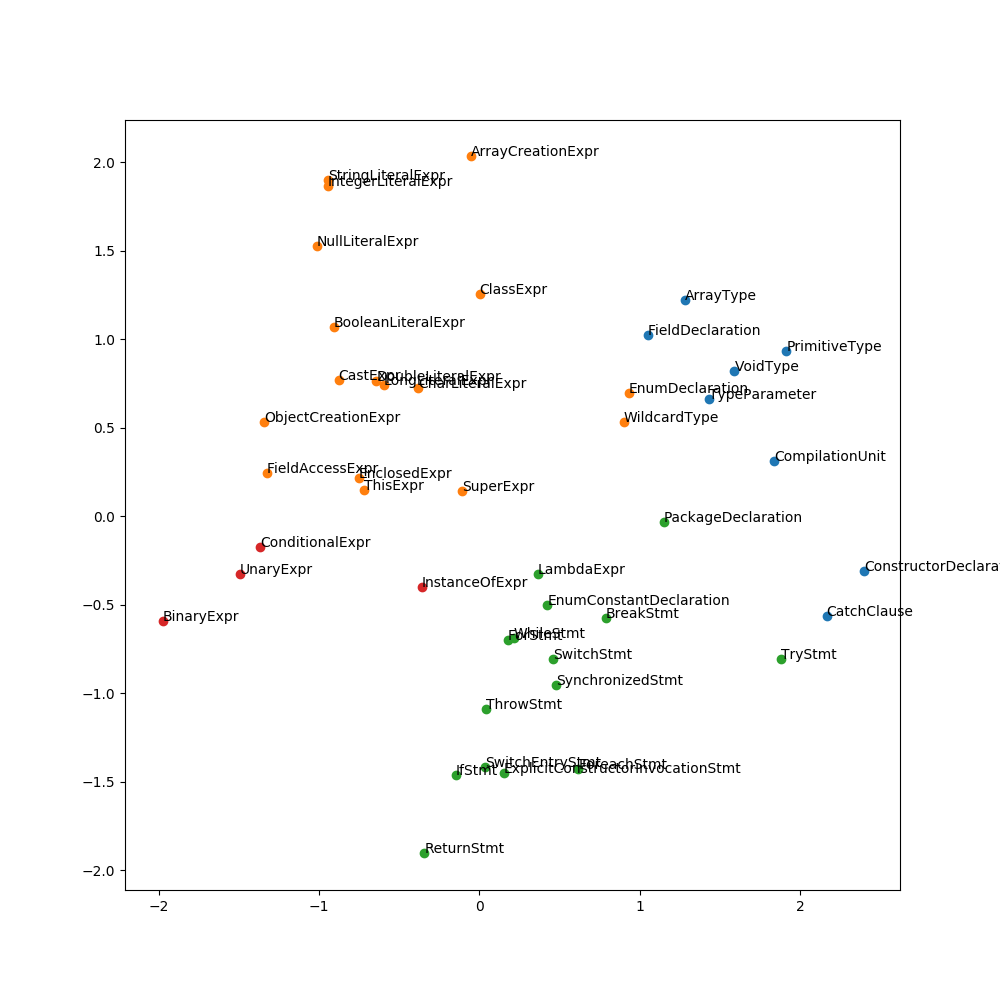
\includegraphics[height=9cm]{images/java-embeddings.png}
  \caption{\label{fig:java-embeddings}Java clustered embedding 2D projection for vocabulary without
  values}
\end{figure}

\begin{figure}
  \centering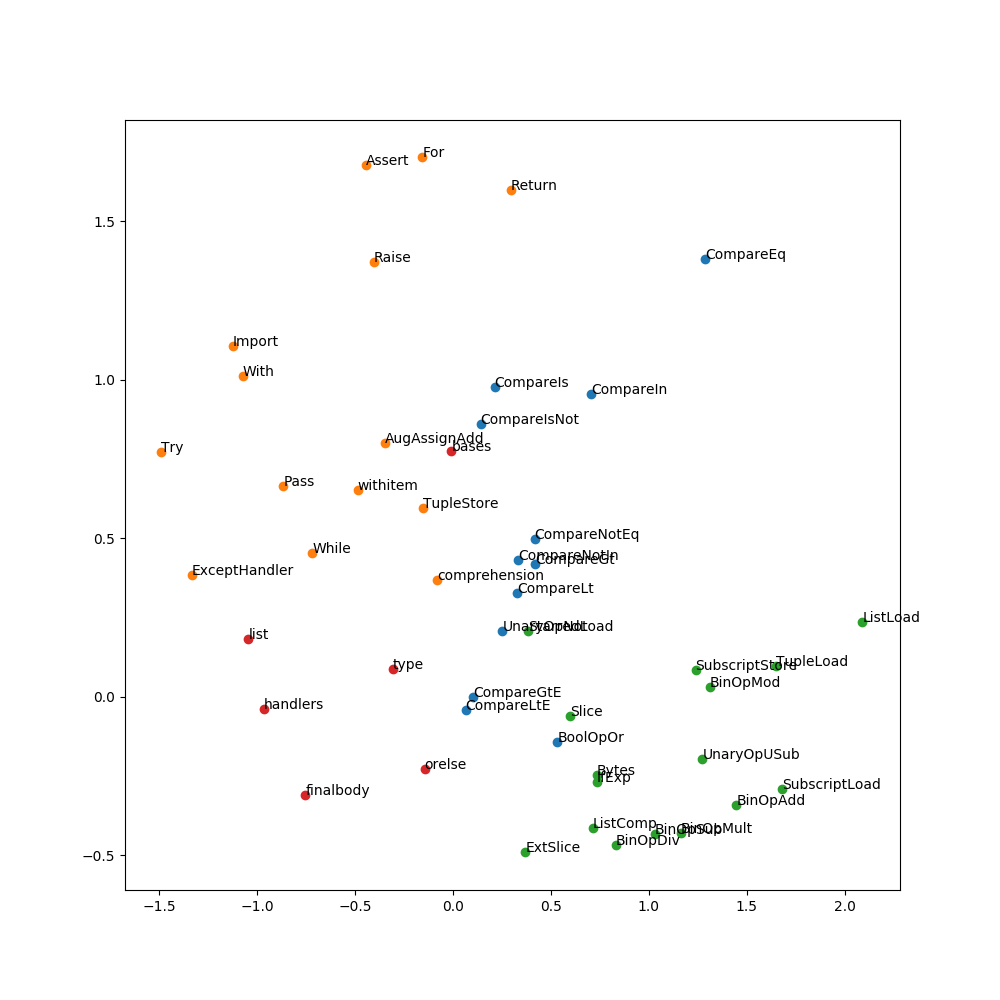
\includegraphics[height=9cm]{images/python-embeddings.png}
  \caption{\label{fig:python-embeddings}Python clustered embedding 2D projection for vocabulary without
  values}
\end{figure}

There are a few interesting things to notice in the results we obtained in
figures~\ref{fig:python-embeddings} and~\ref{fig:java-embeddings}. First, the
clustering we obtain seems quite close to what we could expect when thinking
about the different types of tokens present in the AST. For example, for Java,
All the statements are part of the same cluster, and the only expression which
belongs to this cluster is the \lstinline{LambdaExpr}, which was introduced
in recent versions of Java and appears way less often than most other tokens,
which could explain why it was not clustered correctly. The expressions are also
mostly in the same cluster, and literal expressions, such as
\lstinline{IntegerLiteralExpr} and \lstinline{StringLiteralExpr} are close to
each other, while other related tokens such as \lstinline{ThisExpr} and
\lstinline{SuperExpr} are in the same cluster but further away in the vector
space. The results are similar for Python, where most language constructs, such
as \lstinline{While} or \lstinline{Try} are clustered together, while all the
comparison operators are in another cluster.
Another interesting point is the difference in the relationship of the tokens
between both programming languages. In particular, while \lstinline{While} and
\lstinline{For} appear almost at the same point in the vector space for Java,
which means that both tokens are very similar, the same two tokens are
much further away in Python. This seems a reasonable result to obtain as Java's
\lstinline{while} and \lstinline{for} are indeed interchangeable, while in
Python, these two constructs have different semantics.
